\documentclass[11pt,letterpaper,article]{memoir}
\usepackage[utf8]{inputenc}
\usepackage[T1]{fontenc}
\usepackage{microtype}
\usepackage[dvips]{graphicx}
\usepackage{xcolor}
\usepackage{times}

\usepackage{enumitem}
\setlist[description]{style=nextline}

\usepackage[
breaklinks=true,colorlinks=true,
linkcolor=blue,urlcolor=blue,citecolor=blue,% PDF VIEW
%linkcolor=black,urlcolor=black,citecolor=black,% PRINT
bookmarks=true,bookmarksopenlevel=2]{hyperref}

\usepackage{geometry}
% PDF VIEW
% \geometry{total={210mm,297mm},
% left=25mm,right=25mm,%
% bindingoffset=0mm, top=25mm,bottom=25mm}
% PRINT
\geometry{total={210mm,297mm},
left=20mm,right=20mm,
bindingoffset=10mm, top=25mm,bottom=25mm}

\OnehalfSpacing
%\linespread{1.3}

%%% CHAPTER'S STYLE
%\chapterstyle{bianchi}
%\chapterstyle{ger}
%\chapterstyle{madsen}
%\chapterstyle{ell}

%%% STYLE OF SECTIONS, SUBSECTIONS, AND SUBSUBSECTIONS
\setsecheadstyle{\Large\bfseries\sffamily\raggedright}
\setsubsecheadstyle{\large\bfseries\sffamily\raggedright}
\setsubsubsecheadstyle{\bfseries\sffamily\raggedright}


%%% STYLE OF PAGES NUMBERING
%\pagestyle{companion}\nouppercaseheads 
%\pagestyle{headings}
%\pagestyle{Ruled}
\pagestyle{plain}
\makepagestyle{plain}
\makeevenfoot{plain}{\thepage}{}{}
\makeoddfoot{plain}{}{}{\thepage}
\makeevenhead{plain}{}{}{}
\makeoddhead{plain}{}{}{}

\maxsecnumdepth{subsection} % chapters, sections, and subsections are numbered
\maxtocdepth{subsection} % chapters, sections, and subsections are in the Table of Contents

\newcommand{\name}{PROGRAM_NAME}
\newcommand{\version}{0.1}
\newcommand{\email}{eric.tytell@tufts.edu}

\setlength{\parindent}{0em}



%%%---%%%---%%%---%%%---%%%---%%%---%%%---%%%---%%%---%%%---%%%---%%%---%%%

\begin{document}

\thispagestyle{empty}

{%%%
%\sffamily
\centering
\Large

\vspace*{\fill}

{\huge
\name{} \version \\
}

{\LARGE
User manual \\
\vspace{2.5cm}
David Buckingham \\
Eric Tytell \\
Cassandra Donatelli \\
Margo \\
}
\vspace*{\fill}

}

\cleardoublepage

\tableofcontents*

\clearpage


\section{Copyright and License}

\name{}: a tool for collecting IMU measurements.
Copyright (C) 2017 Author(s)????????/

This program is free software: you can redistribute it and/or modify
it under the terms of the GNU General Public License as published by
the Free Software Foundation, either version 3 of the License, or
(at your option) any later version.

This program is distributed in the hope that it will be useful,
but WITHOUT ANY WARRANTY; without even the implied warranty of
MERCHANTABILITY or FITNESS FOR A PARTICULAR PURPOSE.  See the
GNU General Public License for more details.

You should have received a copy of the GNU General Public License
along with this program.  If not, see <http://www.gnu.org/licenses/>.

\section{Introduction}


\section{Hardware}

\name{} interconnects three pieses of computational hardware:
\begin{enumerate}
  \item a PC
  \item an Arduino
  \item between 1 and 3 Inertial Measurement Units (IMUs)
\end{enumerate}

\subsection{PC}
\name{} has been tested on PCs running Linux (Linux Mint 18 Sarah), macOS (Need to test this and
put version), and Windows (Version??). It uses multi-threading and will perform
best if multiple processing units (cores) are available.

\subsection{Arduino}
\name{} has been tested with an Arduino UNO. It is expected to work on other models having
the same clock speed (16MHz) and sufficient storage.

\subsection{IMUs}
The mpu9250 by InvenSense is nine-axis (gyroscope, accelerometer, compas) motion tracking device.







\section{Installation}

\name{} requires Python3.

We recommend using pip to install \name{}:
\url{https://pypi.python.org/pypi/pip}

\# pip install --upgrade pip
\# pip install \name

Pip will automatically install any of the following dependencies if needed:
\begin{itemize}
\item h5py
\item numpy
\item pyqtgraph
\item pyserial
\item pyqt5
\end{itemize}


\subsection{Arduino code}

\subsubsection{Arduino IDE}
Downlaod and install the Arduino IDE.
The software can be downloaded from:
https://www.arduino.cc/en/Main/Software.
Alternatively, Arduino can be installed on Debian systems with:
\# apt-get install arduino-core

\subsubsection{Install \name{} on the Arduino}
\label{sec:installarduinocode}

Install the file \texttt{am\_tx/am\_tx.ino} on the Arduino.
This can be accomplished using the Arduino IDE graphical user interface.

Alternatively, using Arduino IDE version 1.5.0 or later,
the Arduino can be programmed directly from the command line:
\texttt{\# arduino upload am\_tx/am\_tx.ino}
For more information, see:
\href{https://github.com/arduino/Arduino/blob/master/build/shared/manpage.adoc}
{https://github.com/arduino/Arduino/blob/master/build/shared/manpage.adoc}

\section{Equipment setup}

\subsection{IMUs}
Wiring diagram...

\subsection{Arduino}
To ensure adequate power for the Arduino and IMUs, it is recommended to power
the Arduino with an external power source instead of relying on the USB port.

\section{Collecting data}

To begin collecting data, press the ``record'' button.


\subsection{Data buffer}


\subsection{Trigger}

Optionally, a trigger attached to the Arduino (Section \ref{sec:wiring}) can be
used to stop recording.  If the ``use trigger'' checkbox is not checked, the
trigger is ignored. Otherwise, if an ``active'' trigger is detected, recording
will stop, i.e., the same effect as pressing the ``stop'' button during
recording. If you attempt to begin recording while the ``use trigger'' checkbox
is checked and the trigger is ``active'', the recording end as soon as it starts
with zero data stored.

If the ``invert trigger'' checkbox is not checked, the trigger is considered
``active'' when the associated Arduino pin is set high. If the ``invert
trigger'' checkbox is checked, the trigger is considered ``active'' when the
associated Arduino pin is set low.

If there is nothing setting the current on the Arduino pin associated with the
trigger (i.e. if no trigger is connected), then the value of the pin is
undefined.  Thus, to ensure reliable behavior, the ``use trigger'' checkbox
should not be checked unless there is a trigger connected to the Arduino.

\begin{figure}[]
    \begin{center}
        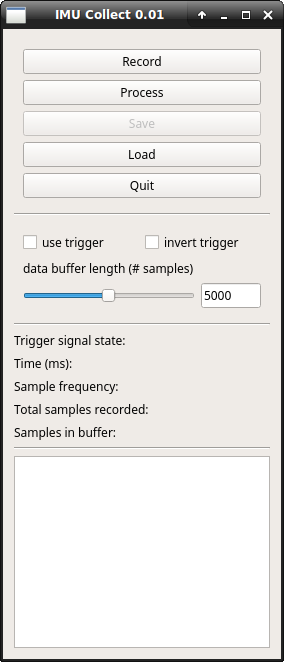
\includegraphics[width=.45\textwidth]{screenshot_0_imu}
    \end{center}
    \caption{Control panel} 
\end{figure}

\begin{figure}[]
    \begin{center}
        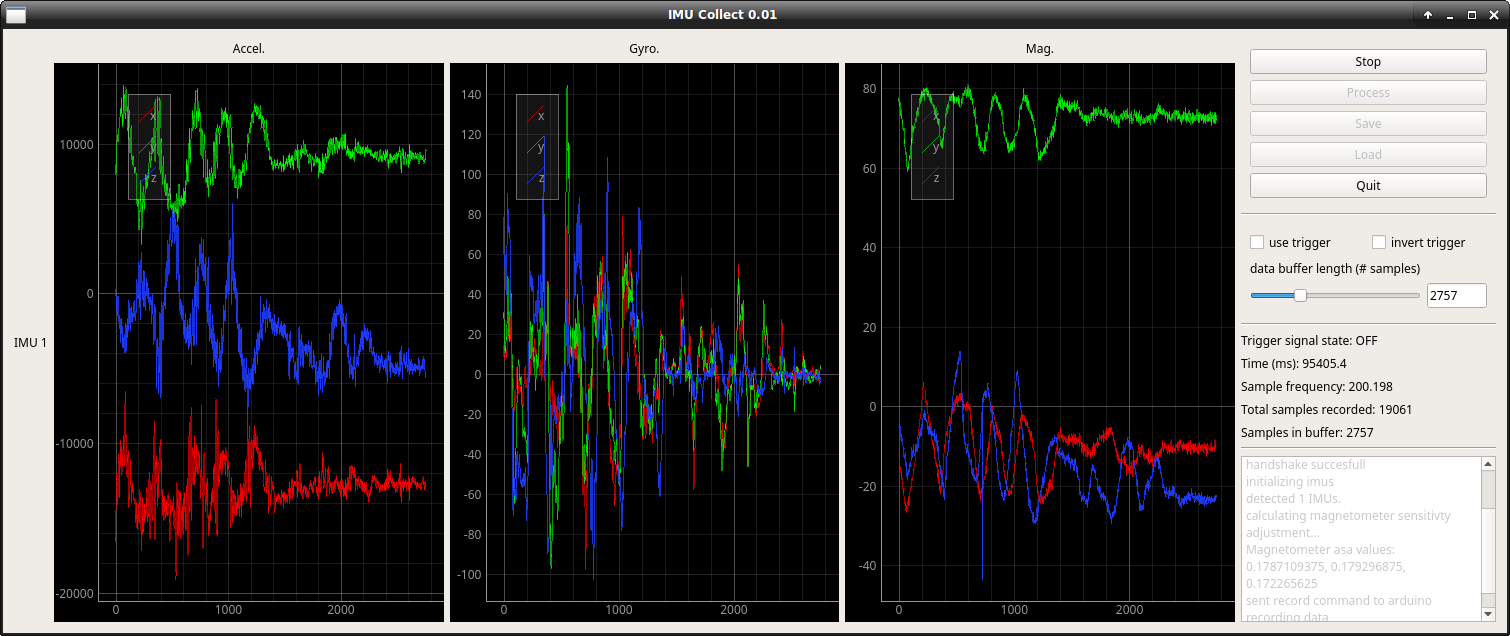
\includegraphics[width=.45\textwidth]{screenshot_1_imu}
    \end{center}
    \caption{Collecting data from a single IMU} 
\end{figure}





\section{Processing data}

\section{Saving and loading}
\subsection{.csv file format}
\label{sec:savingloading}

\section{Settings}

\section{Troubleshooting}

\subsection{Error messages}

\begin{description}
\item[invalid csv file] The program attempted to read a .csv file, but the
format of the data in the file was not valid. See Section
\ref{sec:savingloading} for a description of the .csv file format used by
\name{}.

\item[invalid file type: ...]
\item[rx failed, no data read from serial]
\item[no Arduino found]
\item[failed to create connection]
\item[handshake failed]
\item[no connection, aborting]

\item[unable to determine number of IMUs, aborting] The program failed to
determine how many IMUs are attached to the Arduino. After the Arduino is
initialized, it attempts to determine the number of IMUs by sending a WHOAMI
request while signaling each of the three legal chip select pins (Section
\ref{sec:wiring}). It then sends a message to the PC reporting the number of
IMUs detected. This error is reported if the PC program sends a command to the
Arduino to initialize, but does not receive a message reporting the number of
IMUs detected. Make sure that any IMUs are correctly wired to the Arduino
(Section \ref{sec:wiring}) and that the correct code is installed on the Arduino
(Section \ref{sec:installarduinocode}), and try resetting the Arduino.

\item[no IMUs detected, aborting]

\item[ASA read failed, using 1 adjustment]

\item[Sample packet too short: ...]


\end{description}







%\bibliographystyle{unsrt}
%\bibliography{sample}

\end{document}

